\documentclass{beamer}

\usepackage{fourier} 
\usepackage{pifont,mdframed}

\definecolor{celestialblue}{rgb}{0.29, 0.59, 0.82}

\newenvironment{warning}
  {\par\begin{mdframed}[linewidth=1pt,linecolor=celestialblue]%
    \begin{list}{}{\leftmargin=1cm
                   \labelwidth=\leftmargin}\item[\Large\danger]}
               {\end{list}\end{mdframed}\par}


\title{Building a Collaborative Culture \\ A Grounded Theory of Well Succeeded DevOps \\ Adoption in Practice}

\author{Welder Pinheiro Luz and Gustavo Pinto and Rodrigo Bonif\'{a}cio}

\begin{document}

\begin{frame}
 \titlepage
\end{frame}

\begin{frame}

  \centering{
    \huge{research context} 
  }
\end{frame}


\begin{frame}
  \frametitle{Brazilian Federal Court of Accounts}

  \begin{block}{Current situation}
  \begin{itemize}
    \item JEE architecture 
    \item shared data model
    \item clear separation between development and production teams
    \item rigid time frames for publishing software assets (once a week)  
  \end{itemize}
  \end{block}
  
\end{frame}

\begin{frame}
  \begin{center}
    \begin{huge}
      well known problems 
    \end{huge}
  \end{center}
  \pause
  
  \begin{warning}
    Use of agile development practices, though expected delays
    for making the software available for acceptance
    testing and production environments. 
  \end{warning}
  
\end{frame}


\begin{frame}
  \begin{center}
    \begin{huge}
      well known problems 
    \end{huge}
  \end{center}
  \pause
  
  \begin{warning}
    ``Although it works at the development environment, it does not
      work at the acceptance testing and production environments''. \pause
      ``It must be a bug of the system, so the development team must
      take care of it'' 
  \end{warning}
  
\end{frame}

\begin{frame}

  Let's try to fix this issue using a {\color{blue}DevOps} approach!!!
  
\end{frame}


\begin{frame}
 \centering{
    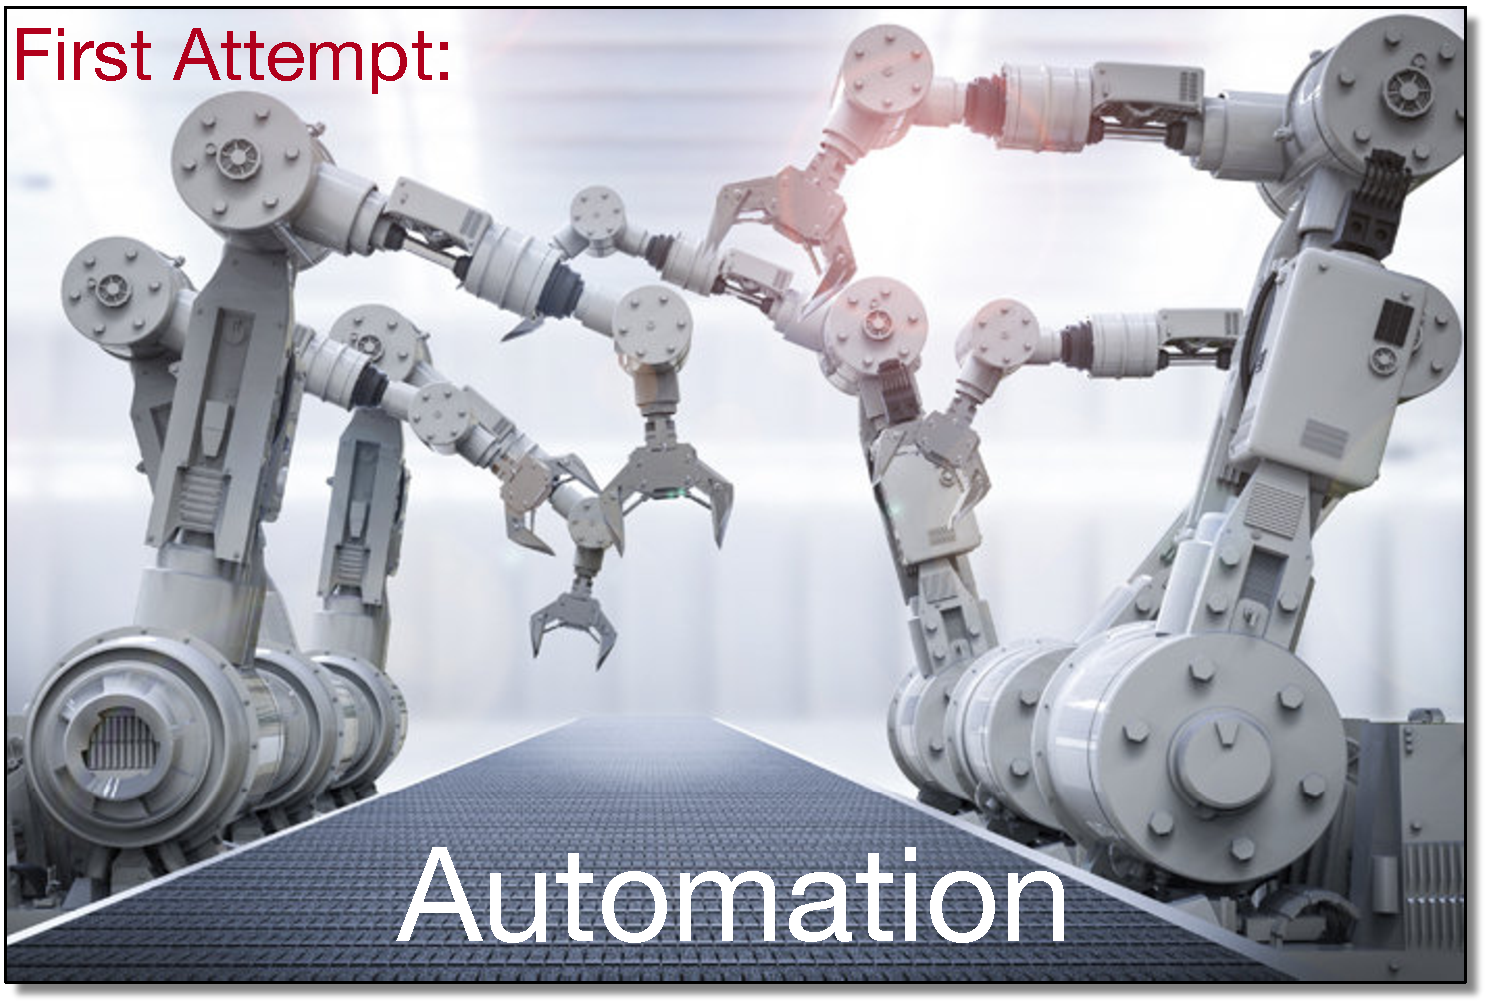
\includegraphics[scale=0.45]{images/automation}
 }
\end{frame}

\begin{frame}
  \centering{
    
\includegraphics[scale=0.5]{images/failed}
  }
\end{frame}

\begin{frame}
  \centering{
    
\includegraphics[scale=0.5]{images/research}
  }
\end{frame}

\begin{frame}

  \begin{description}
   \item[goal:] understand and characterize DevOps
   \item[method:] grounded theory + action research 
  \end{description}
\end{frame}

\end{document}
